\documentclass[aspectratio=169]{beamer}
\usetheme{metropolis}
\usepackage{booktabs}
\usepackage{listings}
\usepackage{xcolor}
\usepackage{tikz}
\usepackage{pgfplots}
\pgfplotsset{compat=1.18}

% Color scheme - dark theme
\definecolor{bgdark}{HTML}{1a1a2e}
\definecolor{accent}{HTML}{e94560}
\definecolor{accent2}{HTML}{0f3460}
\definecolor{textlight}{HTML}{eaeaea}
\definecolor{codebg}{HTML}{16213e}
\definecolor{codegreen}{HTML}{00ff88}

\setbeamercolor{background canvas}{bg=bgdark}
\setbeamercolor{normal text}{fg=textlight}
\setbeamercolor{frametitle}{fg=textlight,bg=accent2}
\setbeamercolor{title}{fg=textlight}
\setbeamercolor{progress bar}{fg=accent}
\setbeamercolor{alerted text}{fg=accent}

% Code listings style
\lstset{
    basicstyle=\ttfamily\tiny,
    backgroundcolor=\color{codebg},
    keywordstyle=\color{accent},
    stringstyle=\color{codegreen},
    commentstyle=\color{gray},
    breaklines=true,
    frame=single,
    rulecolor=\color{accent2}
}

\title{Profiling \& Optimizing GPU Training Pipelines}
\subtitle{A Deep Dive into nanoTabPFN Data Loading Bottlenecks}
\author{CUDA Performance Engineering}
\date{January 2026}

\begin{document}

\begin{frame}
\titlepage
\end{frame}

%--------------------------------------------------
\section{The Problem}
%--------------------------------------------------

\begin{frame}{nanoTabPFN: Context}
\textbf{What is it?}
\begin{itemize}
    \item A \alert{TabPFN} (Tabular Prior-Fitted Network) implementation
    \item Pre-trained transformer for tabular classification
    \item Training uses HDF5 prior dumps (300k synthetic datasets)
    \item Each sample: up to 150 rows $\times$ 5 features
\end{itemize}

\vspace{0.5em}
\textbf{The Question:} How do we make training faster?

\vspace{0.5em}
\textbf{Hardware:} NVIDIA A100-SXM4-80GB
\end{frame}

\begin{frame}{Initial Baseline: train.py}
\begin{columns}
\begin{column}{0.5\textwidth}
\textbf{Original Implementation:}
\begin{itemize}
    \item Standard h5py reads
    \item Synchronous \texttt{.to(device)} transfers
    \item No profiling instrumentation
    \item Default PyTorch settings
\end{itemize}
\end{column}
\begin{column}{0.5\textwidth}
\begin{lstlisting}[language=Python]
# Original dataloader
with h5py.File(filename, "r") as f:
    for _ in range(num_steps):
        x = torch.from_numpy(
            f["X"][ptr:end]
        )
        y = torch.from_numpy(
            f["y"][ptr:end]
        )
        yield dict(
            x=x.to(device),  # Sync
            y=y.to(device),  # Sync
        )
\end{lstlisting}
\end{column}
\end{columns}
\end{frame}

%--------------------------------------------------
\section{Profiling}
%--------------------------------------------------

\begin{frame}{Adding Profiling Instrumentation}
\textbf{Step 1:} Add PyTorch Profiler to \texttt{train.py}

\begin{lstlisting}[language=Python]
from torch.profiler import profile, ProfilerActivity

with profile(
    activities=[ProfilerActivity.CPU, ProfilerActivity.CUDA],
    record_shapes=True,
    profile_memory=True,
) as prof:
    model, history = train(model, prior, lr=4e-3)

print(prof.key_averages().table(sort_by="cuda_time_total"))
print(prof.key_averages().table(sort_by="cpu_time_total"))
\end{lstlisting}

\vspace{0.5em}
\textbf{Key additions:}
\begin{itemize}
    \item \texttt{--profile} flag for profiling mode
    \item \texttt{--steps} to control training duration
    \item \texttt{--batch-size} for experimentation
\end{itemize}
\end{frame}

\begin{frame}{Baseline Profile Results (100 steps)}
\textbf{Configuration:} Batch size 6, 5000 rows/sample, A100 80GB

\vspace{0.5em}
\begin{table}
\centering
\footnotesize
\begin{tabular}{lrr}
\toprule
\textbf{Metric} & \textbf{Value} & \textbf{Interpretation} \\
\midrule
Total time & 68.75s & Slow \\
Steps/sec & 1.5 & Low throughput \\
ms/step & 687.51 & High latency \\
\midrule
cudaMemcpyAsync (CPU) & 44,084ms & \alert{76.8\% of CPU time!} \\
aten::copy\_ (CPU) & 44,352ms & Data transfer bottleneck \\
aten::bmm (CUDA) & 32,509ms & Attention compute \\
\bottomrule
\end{tabular}
\end{table}

\vspace{0.5em}
\textbf{Diagnosis:} \alert{CPU spends 77\% of time on data transfers}
\end{frame}

\begin{frame}{Baseline: CPU Operations Breakdown}
\begin{center}
\begin{tikzpicture}
\pie[
    radius=2.5,
    color={accent!80, accent2!80, gray!60, textlight!30},
    text=legend,
    explode={0.1, 0, 0, 0}
]{
    76.78/cudaMemcpyAsync (sync),
    12.33/cudaMalloc,
    6.91/aten::bmm,
    3.98/Other
}
\end{tikzpicture}
\end{center}

\vspace{0.5em}
\textbf{The bottleneck is clear:} Synchronous CPU$\rightarrow$GPU transfers dominate
\end{frame}

%--------------------------------------------------
\section{Optimizations}
%--------------------------------------------------

\begin{frame}{Optimization Strategy: train\_optimized.py}
\textbf{Target:} Eliminate data transfer bottlenecks

\vspace{0.5em}
\begin{enumerate}
    \item \textbf{TF32 \& cuDNN Benchmark} -- Faster matmuls on Ampere+
    \item \textbf{Pinned Memory} -- Page-locked CPU memory for faster DMA
    \item \textbf{Non-blocking Transfers} -- Async CPU$\rightarrow$GPU copies
    \item \textbf{CUDA Streams} -- Overlap transfer with compute
    \item \textbf{Double Buffering} -- Prefetch next batch while computing
    \item \textbf{GPU Direct Storage (GDS)} -- Disk$\rightarrow$VRAM, bypass CPU
\end{enumerate}
\end{frame}

\begin{frame}{Optimization 1: TF32 \& Performance Flags}
\begin{lstlisting}[language=Python]
# Enable TF32 for Ampere+ GPUs (2x faster matmuls)
torch.backends.cuda.matmul.allow_tf32 = True
torch.backends.cudnn.allow_tf32 = True
torch.backends.cudnn.benchmark = True  # auto-tune convolutions

# Faster gradient zeroing
optimizer.zero_grad(set_to_none=True)
\end{lstlisting}

\vspace{0.5em}
\textbf{Impact:}
\begin{itemize}
    \item TF32: 19-bit mantissa (vs FP32's 24-bit) with tensor cores
    \item cuDNN benchmark: finds fastest algorithm for current shapes
    \item \texttt{set\_to\_none=True}: avoids memset, uses None directly
\end{itemize}
\end{frame}

\begin{frame}{Optimization 2: Pinned Memory + Non-blocking Transfers}
\begin{lstlisting}[language=Python]
# Before: Synchronous transfer
x = torch.from_numpy(x_np).to(device)  # Blocks CPU

# After: Pinned memory + async transfer
x = torch.from_numpy(x_np).pin_memory().to(device, non_blocking=True)
\end{lstlisting}

\vspace{0.5em}
\textbf{Why this works:}
\begin{itemize}
    \item \texttt{pin\_memory()}: Page-locked memory, DMA-accessible
    \item \texttt{non\_blocking=True}: Returns immediately, transfer happens in background
    \item Requires CUDA streams to actually overlap
\end{itemize}
\end{frame}

\begin{frame}{Optimization 3: CUDA Streams + Double Buffering}
\begin{lstlisting}[language=Python]
class PriorDumpDataLoader:
    def __init__(self, ...):
        self.transfer_stream = torch.cuda.Stream()
    
    def __iter__(self):
        vram_buffer = [self._load_to_vram(f) for _ in range(prefetch)]
        
        for step in range(num_steps):
            batch = vram_buffer.pop(0)  # Already in VRAM
            
            # Prefetch next batch on separate stream
            with torch.cuda.stream(self.transfer_stream):
                next_batch = self._load_to_vram(f)
            vram_buffer.append(next_batch)
            
            # Sync before yielding
            torch.cuda.current_stream().wait_stream(self.transfer_stream)
            yield batch
\end{lstlisting}
\end{frame}

\begin{frame}{Optimization 4: GPU Direct Storage (kvikio)}
\begin{lstlisting}[language=Python]
import kvikio
import cupy as cp

class GDSDataLoader:
    """Disk -> GPU VRAM, bypassing CPU entirely"""
    
    def _iter_gds(self):
        with h5py.File(self.filename, "r") as f:
            # Allocate GPU buffers
            x_gpu = cp.empty((batch_size, max_seq, num_features), dtype=cp.float32)
            
            # Read directly to GPU (cupy handles GDS)
            x_gpu[:] = cp.asarray(f["X"][ptr:end])
            
            # Zero-copy to PyTorch
            x = torch.as_tensor(x_gpu, device=self.device)
            yield dict(x=x, y=y, ...)
\end{lstlisting}

\vspace{0.5em}
\textbf{Note:} True GDS requires raw binary files; HDF5 still involves some CPU
\end{frame}

%--------------------------------------------------
\section{Results}
%--------------------------------------------------

\begin{frame}{Optimized Profile Results (100 steps)}
\textbf{Configuration:} Batch size 6, 5000 rows/sample, A100 80GB, GDS enabled

\vspace{0.5em}
\begin{table}
\centering
\footnotesize
\begin{tabular}{lrrr}
\toprule
\textbf{Metric} & \textbf{Baseline} & \textbf{Optimized} & \textbf{Speedup} \\
\midrule
Total time & 68.75s & 45.30s & \textbf{1.52$\times$} \\
Steps/sec & 1.5 & 2.2 & \textbf{1.47$\times$} \\
ms/step & 687.51 & 453.00 & \textbf{1.52$\times$} \\
\midrule
cudaMemcpyAsync (CPU) & 44,084ms & 268ms & \textbf{164$\times$} \\
aten::copy\_ (CPU) & 44,352ms & 4,425ms & \textbf{10$\times$} \\
\bottomrule
\end{tabular}
\end{table}

\vspace{0.5em}
\textbf{Key win:} Data transfer time reduced from 44s to 0.27s
\end{frame}

\begin{frame}{Where Did the Time Go?}
\begin{columns}
\begin{column}{0.5\textwidth}
\textbf{Baseline CPU Time:}
\begin{itemize}
    \item \alert{76.78\%} cudaMemcpyAsync
    \item 12.33\% cudaMalloc
    \item 1.12\% cudaLaunchKernel
    \item 9.77\% Other
\end{itemize}
\end{column}
\begin{column}{0.5\textwidth}
\textbf{Optimized CPU Time:}
\begin{itemize}
    \item \alert{46.91\%} Command Buffer Full
    \item 21.47\% cudaLaunchKernel
    \item 11.22\% cudaMalloc
    \item 8.85\% aten::copy\_
\end{itemize}
\end{column}
\end{columns}

\vspace{1em}
\textbf{New bottleneck:} GPU is now \textit{saturated}---the command buffer is full!

This means the GPU can't keep up with the kernel submissions.
\end{frame}

\begin{frame}{Memory Transfer Comparison}
\begin{table}
\centering
\begin{tabular}{lrr}
\toprule
\textbf{Operation} & \textbf{Baseline} & \textbf{Optimized} \\
\midrule
aten::to (CPU time) & 44,240ms & 109ms \\
cudaMemcpyAsync (CPU time) & 44,084ms & 268ms \\
aten::copy\_ (CPU time) & 44,352ms & 4,425ms \\
\midrule
\textbf{Total H2D overhead} & \alert{44s} & \textbf{0.27s} \\
\textbf{Reduction} & --- & \textbf{99.4\%} \\
\bottomrule
\end{tabular}
\end{table}

\vspace{0.5em}
The data loading is no longer the bottleneck.
\end{frame}

%--------------------------------------------------
\section{Scaling Analysis}
%--------------------------------------------------

\begin{frame}{Scaling with Data Size}
\textbf{Test data generated with:}
\begin{lstlisting}[language=bash]
python generate_synthetic_data.py --scale 0.1 --rows 5000
# -> 30k_5000x5_2.h5 (3.6 GB)
\end{lstlisting}

\vspace{0.5em}
\begin{table}
\centering
\begin{tabular}{lrrr}
\toprule
\textbf{Dataset} & \textbf{Samples} & \textbf{Rows/Sample} & \textbf{Size} \\
\midrule
Original & 300k & 150 & 989 MB \\
Scaled (0.1$\times$, 5000 rows) & 30k & 5000 & 3.6 GB \\
\bottomrule
\end{tabular}
\end{table}

\vspace{0.5em}
\textbf{Key insight:} Longer sequences (5000 vs 150 rows) stress attention's $O(n^2)$ memory
\end{frame}

\begin{frame}{Memory Scaling}
\textbf{Peak CUDA Memory:} 72.3 GiB / 80 GiB (90\% utilization)

\vspace{0.5em}
\begin{table}
\centering
\begin{tabular}{lr}
\toprule
\textbf{Metric} & \textbf{Value} \\
\midrule
Total Allocated & 12,864 GiB (cumulative) \\
Peak Usage & 72,326 MiB \\
GPU Reserved & 79,890 MiB \\
cudaMalloc retries & 5 \\
\bottomrule
\end{tabular}
\end{table}

\vspace{0.5em}
\textbf{Attention memory:} $O(batch \times heads \times seq^2)$

With 5000 rows: $6 \times 4 \times 5000^2 \times 4$ bytes $\approx$ 2.4 GB per layer
\end{frame}

\begin{frame}{What's Next? Further Optimizations}
\textbf{Now that data loading is solved, remaining bottlenecks:}

\vspace{0.5em}
\begin{enumerate}
    \item \textbf{torch.compile()} -- Fuse kernels, reduce launch overhead
    \begin{itemize}
        \item Currently disabled due to profiling overhead
        \item Would reduce 51k kernel launches significantly
    \end{itemize}
    
    \item \textbf{Flash Attention} -- $O(n)$ memory instead of $O(n^2)$
    \begin{itemize}
        \item Critical for long sequences (5000+ rows)
        \item Would allow larger batch sizes
    \end{itemize}
    
    \item \textbf{Gradient Checkpointing} -- Trade compute for memory
    \begin{itemize}
        \item Recompute activations during backward pass
        \item 2$\times$ compute, 10$\times$ less memory
    \end{itemize}
\end{enumerate}
\end{frame}

\begin{frame}{Estimated Scaling}
\begin{center}
\begin{tikzpicture}
\begin{axis}[
    xlabel={Sequence Length (rows)},
    ylabel={Time per Step (ms)},
    xmode=log,
    ymode=log,
    grid=major,
    width=0.8\textwidth,
    height=0.6\textheight,
    legend pos=north west,
    xmin=100, xmax=10000,
    ymin=10, ymax=10000,
]
\addplot[color=accent, thick, mark=*] coordinates {
    (150, 10)
    (500, 50)
    (1000, 150)
    (5000, 453)
};
\addlegendentry{Optimized (measured)}

\addplot[color=gray, dashed, thick] coordinates {
    (150, 20)
    (500, 100)
    (1000, 300)
    (5000, 687)
};
\addlegendentry{Baseline (estimated)}

\end{axis}
\end{tikzpicture}
\end{center}
\end{frame}

%--------------------------------------------------
\section{Takeaways}
%--------------------------------------------------

\begin{frame}{Summary}
\textbf{Profiling-Driven Optimization:}
\begin{enumerate}
    \item \textbf{Profile first} -- Don't guess, measure
    \item \textbf{Find the bottleneck} -- 77\% on data transfers!
    \item \textbf{Target the bottleneck} -- Pinned memory, streams, GDS
    \item \textbf{Re-profile} -- Verify improvement, find next bottleneck
\end{enumerate}

\vspace{1em}
\textbf{Results:}
\begin{itemize}
    \item \textbf{1.52$\times$} overall speedup
    \item \textbf{164$\times$} reduction in cudaMemcpyAsync time
    \item \textbf{99.4\%} reduction in H2D transfer overhead
    \item New bottleneck: GPU compute (which is what we want!)
\end{itemize}
\end{frame}

\begin{frame}{Code Available}
\begin{center}
\Large
\texttt{github.com/stprnvsh/nanoTabPFN}
\end{center}

\vspace{1em}
\textbf{Files:}
\begin{itemize}
    \item \texttt{train.py} -- Baseline with profiling
    \item \texttt{train\_optimized.py} -- All optimizations
    \item \texttt{generate\_synthetic\_data.py} -- Create test data
\end{itemize}

\vspace{1em}
\textbf{Run profiling:}
\begin{lstlisting}[language=bash]
python train.py --profile --steps=100 --batch-size=6
python train_optimized.py --profile --gds --steps=100 --batch-size=6
\end{lstlisting}
\end{frame}

\begin{frame}[standout]
Questions?
\end{frame}

\end{document}

